\documentclass[Main.tex]{subfiles} 
\begin{document}

\subsection{Sprint 4}
Sprint 4 blev kort, grundet p�skeferie. Men sprintet gik prim�rt ud p� udvikling af programmer og algoritmer. 
Meget f� emner blev f�rdiggjort, da mange af emnerne havde s�rdeles store udfordringer, der ikke var forudset. 
\\
\begin{wrapfigure}{r}{0.6\textwidth}
	\vspace{-20pt}
    \centering
	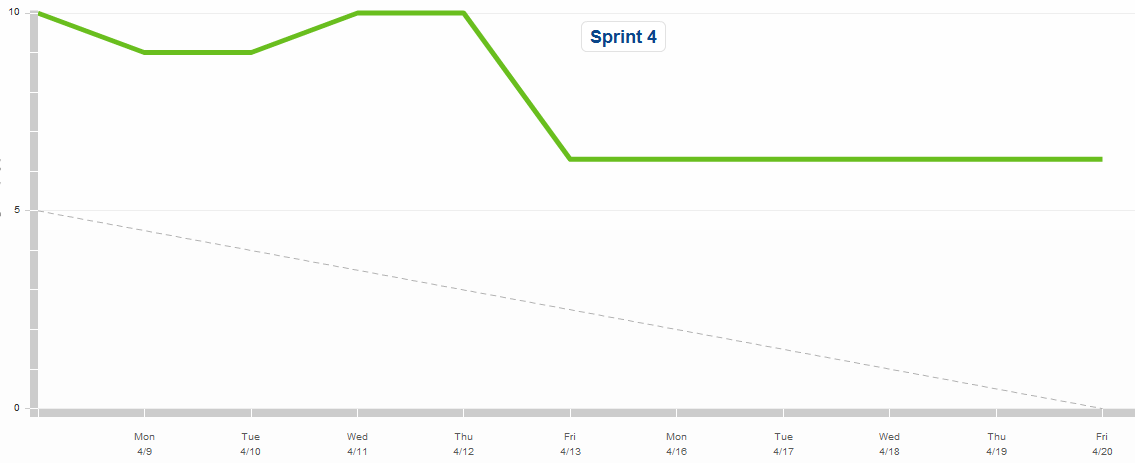
\includegraphics[scale=0.25]{Billeder/Sprint4_burn.png}
	\vspace{-20pt}
	\caption{Burndown chart for sprint 4}
  \label{fig:sprint4}
  \vspace{-10pt}
\end{wrapfigure}
F�lgende gav de st�rste problemer:

	\begin{itemize}
	\item Algoritme til at kunne rykke p� transportb�nd.
	\item Database synkronisering.
	\item Det funktionelle programs funktioner i en sekvens.
	\item V�gten fejlede grundet defekt fumlebr�t.
	\end{itemize}

Det resulterede i, at sprintet og flere af dets opgaver blev flyttet til Sprint 5.

\end{document}